% Font options: 10pm, 11pt, 12pt
% Align headings left instead of center: nocenter
\documentclass[xcolor=x11names,compress]{beamer}\usepackage[]{graphicx}\usepackage[]{color}
%% maxwidth is the original width if it is less than linewidth
%% otherwise use linewidth (to make sure the graphics do not exceed the margin)
\makeatletter
\def\maxwidth{ %
  \ifdim\Gin@nat@width>\linewidth
    \linewidth
  \else
    \Gin@nat@width
  \fi
}
\makeatother

\definecolor{fgcolor}{rgb}{0.345, 0.345, 0.345}
\newcommand{\hlnum}[1]{\textcolor[rgb]{0.686,0.059,0.569}{#1}}%
\newcommand{\hlstr}[1]{\textcolor[rgb]{0.192,0.494,0.8}{#1}}%
\newcommand{\hlcom}[1]{\textcolor[rgb]{0.678,0.584,0.686}{\textit{#1}}}%
\newcommand{\hlopt}[1]{\textcolor[rgb]{0,0,0}{#1}}%
\newcommand{\hlstd}[1]{\textcolor[rgb]{0.345,0.345,0.345}{#1}}%
\newcommand{\hlkwa}[1]{\textcolor[rgb]{0.161,0.373,0.58}{\textbf{#1}}}%
\newcommand{\hlkwb}[1]{\textcolor[rgb]{0.69,0.353,0.396}{#1}}%
\newcommand{\hlkwc}[1]{\textcolor[rgb]{0.333,0.667,0.333}{#1}}%
\newcommand{\hlkwd}[1]{\textcolor[rgb]{0.737,0.353,0.396}{\textbf{#1}}}%
\let\hlipl\hlkwb

\usepackage{framed}
\makeatletter
\newenvironment{kframe}{%
 \def\at@end@of@kframe{}%
 \ifinner\ifhmode%
  \def\at@end@of@kframe{\end{minipage}}%
  \begin{minipage}{\columnwidth}%
 \fi\fi%
 \def\FrameCommand##1{\hskip\@totalleftmargin \hskip-\fboxsep
 \colorbox{shadecolor}{##1}\hskip-\fboxsep
     % There is no \\@totalrightmargin, so:
     \hskip-\linewidth \hskip-\@totalleftmargin \hskip\columnwidth}%
 \MakeFramed {\advance\hsize-\width
   \@totalleftmargin\z@ \linewidth\hsize
   \@setminipage}}%
 {\par\unskip\endMakeFramed%
 \at@end@of@kframe}
\makeatother

\definecolor{shadecolor}{rgb}{.97, .97, .97}
\definecolor{messagecolor}{rgb}{0, 0, 0}
\definecolor{warningcolor}{rgb}{1, 0, 1}
\definecolor{errorcolor}{rgb}{1, 0, 0}
\newenvironment{knitrout}{}{} % an empty environment to be redefined in TeX

\usepackage{alltt}
%\documentclass[xcolor=x11names,compress,handout]{beamer}
\usepackage[]{graphicx}
\usepackage[]{color}
\usepackage{booktabs}
\usepackage{hyperref}
\usepackage{tikz}
\usepackage{multirow}
\usepackage{dcolumn}
\usepackage{bigstrut}
\usepackage{amsmath} 
\usepackage{xcolor,colortbl}
\usepackage{amssymb}
%\newcommand{\done}{\cellcolor{teal}#1}

%% Beamer Layout %%%%%%%%%%%%%%%%%%%%%%%%%%%%%%%%%%
\useoutertheme[subsection=false,shadow]{miniframes}
\useinnertheme{default}
\usefonttheme{serif}
\usepackage{Arev}
\usepackage{pdfpages}

\setbeamerfont{title like}{shape=\scshape}
\setbeamerfont{frametitle}{shape=\scshape, size=\normalsize}

\definecolor{dkblue}{RGB}{0,0,102}

\setbeamercolor*{lower separation line head}{bg=dkblue} 
\setbeamercolor*{normal text}{fg=black,bg=white} 
\setbeamercolor*{alerted text}{fg=red} 
\setbeamercolor*{example text}{fg=black} 
\setbeamercolor*{structure}{fg=black} 
 
\setbeamercolor*{palette tertiary}{fg=black,bg=black!10} 
\setbeamercolor*{palette quaternary}{fg=black,bg=black!10} 

\renewcommand{\(}{\begin{columns}}
\renewcommand{\)}{\end{columns}}
\newcommand{\<}[1]{\begin{column}{#1}}
\renewcommand{\>}{\end{column}}

\AtBeginSection{\frame{\sectionpage}}
\usepackage{xcolor}
\hypersetup{
    colorlinks,
    linkcolor={red!50!black},
    citecolor={blue!50!black},
    urlcolor={blue!80!black}
}

\setbeamertemplate{navigation symbols}{} 
\setbeamertemplate{footline}[frame number]
\setbeamertemplate{caption}{\raggedright\insertcaption\par}

\setbeamersize{text margin left=5pt,text margin right=5pt}

%%%%%%%%%%%%%%%%%%%%%%%%%%%%%%%%%%%%%%%%%%%%%%%%%%


\title{FLS 6441 - Methods III: Explanation and Causation}
\subtitle{Week 8 - Difference-in-Differences}
\author{Jonathan Phillips}
\date{May 2019}
\IfFileExists{upquote.sty}{\usepackage{upquote}}{}
\begin{document}




\frame{\titlepage}

\begin{frame}
\frametitle{Classification of Research Designs}
\footnotesize
\begin{table}[htbp]
  \centering
  \scalebox{0.7}{
    \begin{tabular}{|p{2.2cm}|p{5cm}|c|c|}
    \hline
          &       & \multicolumn{1}{p{2.4cm}|}{\textbf{Independence of Treatment Assignment}} & \multicolumn{1}{p{3cm}|}{\textbf{Researcher Controls Treatment Assignment?}} \bigstrut\\
    \hline
    \multicolumn{1}{|p{2.9cm}|}{\multirow{2}[4]{2.9cm}{\textbf{Controlled Experiments}}} & Field Experiments & \checkmark      & \checkmark  \bigstrut\\
\cline{2-4}          & Survey and Lab Experiments &  \checkmark     & \checkmark \bigstrut\\
    \hline
          &       &       &  \bigstrut\\
    \hline
    \multicolumn{1}{|p{2.9cm}|}{\multirow{3}[6]{2.9cm}{\textbf{Natural Experiments}}} & Natural Experiments &  \checkmark     &  \bigstrut\\
\cline{2-4}          & Instrumental Variables & \checkmark      &  \bigstrut\\
\cline{2-4}          & Discontinuities & \checkmark      &  \bigstrut\\
    \hline
          &       &       &  \bigstrut\\
    \hline
    \multicolumn{1}{|p{2.9cm}|}{\multirow{4}[8]{2.9cm}{\textbf{Observational Studies}}} & Difference-in-Differences &       &  \bigstrut\\
\cline{2-4}          & Controlling for Confounding &       &  \bigstrut\\
\cline{2-4}          & Matching &       &  \bigstrut\\
\cline{2-4}          & Comparative Cases and Process Tracing &       &  \bigstrut\\
    \hline
    \end{tabular}}%
  \label{tab:addlabel}%
\end{table}%
\normalsize
\end{frame}


\section{Difference-in-Differences}

\begin{frame}
\frametitle{Difference-in-Differences}
\begin{itemize}
\item What if we have \textit{NO} variation in treatment that is independent of potential outcomes?
\pause
\item Then we have an \textit{Observational} study
\end{itemize}
\end{frame}

\begin{frame}
\frametitle{Difference-in-Differences}
\begin{itemize}
\item Two types of observational studies:
\end{itemize}
\pause
\begin{enumerate}
\item \textbf{Cross-sectional:} Compare across different units, \textbf{treated} and \textbf{control}
\pause
\begin{itemize}
\item BUT Omitted variable bias
\end{itemize}
\pause
\item \textbf{Time-series:} Compare units \textbf{before} and \textbf{after} treatment
\pause
\begin{itemize}
\item BUT Outcomes might change over time for reasons other than treatment ('Overall Trend Bias')
\end{itemize}
\end{enumerate}
\end{frame}

\begin{frame}
\frametitle{Difference-in-Differences}
\begin{itemize}
\item But each approach also has advantages
\end{itemize}
\pause
\begin{enumerate}
\item \textbf{Cross-sectional:} Compare across different units, \textbf{treated} and \textbf{control}
\pause
\begin{itemize}
\item Allows us to compare units at the same point in time, removing 'Overall Trend Bias'
\end{itemize}
\pause
\item \textbf{Time-series:} Compare units \textbf{before} and \textbf{after} treatment
\pause
\begin{itemize}
\item Allows us to keep the characteristics of the unit the same, removing Omitted Variable Bias
\pause
\item Even \textit{unobserved} characteristics
\end{itemize}
\end{enumerate}
\end{frame}

\begin{frame}
\frametitle{Difference-in-Differences}
\begin{itemize}
\item What if we combine both approaches?
\pause
\item Comparing \textbf{across units} and \textbf{across time}
\pause
\item Removing the risks from both overall trends and omitted variables
\end{itemize}
\end{frame}

\begin{frame}
\frametitle{Difference-in-Differences}
\begin{itemize}
\item Example: How has the Brexit vote affected the UK's growth rate?
\pause
\begin{itemize}
\item Comparing with European growth rates is biased - UK growth is influenced by oil, different labour laws etc.
\pause
\item Comparing before and after the Brexit vote is biased - the world economy improved around the same time as Brexit (coincidentally)
\pause
\item But compare how European growth \textbf{changes} (+0.3\%) and UK growth \textbf{changed} (-0.4\%)
\pause
\item The net effect of Brexit is -0.7\%
\pause
\item That's two differences
\begin{itemize}
\item \textbf{Difference 1:} Between before and after (over time)
\item \textbf{Difference 2:} Between treated and control units
\pause
\end{itemize}
\end{itemize}
\end{itemize}
\end{frame}

\begin{frame}
\frametitle{Difference-in-Differences}
\begin{center}
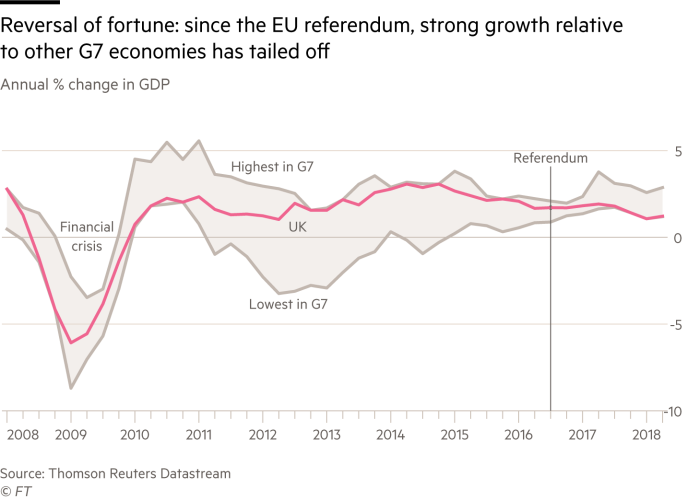
\includegraphics[scale=0.7]{UK_EU_Growth.png}
\end{center}
\end{frame}

\begin{frame}
\frametitle{Difference-in-Differences}
\begin{itemize}
\item But can we really say this was the effect of Brexit?
\end{itemize}
\pause
\begin{enumerate}
\item Maybe the UK was on a different \textbf{unit-specific trend} to the EU before Brexit?
\pause
\begin{itemize}
\item Diff-in-Diff does NOT control for \textbf{time-varying confounders}
\pause
\item We have to check for \textbf{Parallel pre-treatment trends}
\end{itemize}
\item Maybe the UK passed other policies at the same time as Brexit?
\pause
\begin{itemize}
\item We have to check there are no \textbf{compound treatments}
\end{itemize}
\end{enumerate}
\end{frame}

\begin{frame}
\frametitle{Difference-in-Differences}
\footnotesize
\begin{table}[htbp]
  \centering
  \caption{Add caption}
    \begin{tabular}{lcccc}
          & \multicolumn{2}{p{12.43em}}{Balances time-invariant 'fixed' unit characteristics} & \multicolumn{2}{c}{Balances time-varying characteristics} \\
          & \multicolumn{1}{l}{Observed} & \multicolumn{1}{l}{Unobserved} & \multicolumn{1}{l}{Overall trends} & \multicolumn{1}{l}{Unit-specific trends} \\
    Field Experiments & \checkmark     & \checkmark     & \checkmark     & \checkmark \\
    Survey and Lab Experiments & \checkmark     & \checkmark     & \checkmark     & \checkmark \\
          &       &       &       &  \\
    Natural Experiments & \checkmark     & \checkmark     & \checkmark     & \checkmark \\
    Instrumental Variables & \checkmark     & \checkmark     & \checkmark     & \checkmark \\
    Regression Discontinuity & \checkmark     & \checkmark     & \checkmark     & \checkmark \\
          &       &       &       &  \\
    Cross-sectional comparisons & X     & X     & \checkmark     & X \\
    Before-After comparisons & \checkmark     & \checkmark     & X     & X \\
    Difference-in-Differences & \checkmark     & \checkmark     & \checkmark     & X \\
    \end{tabular}%
  \label{tab:addlabel}%
\end{table}%
\normalsize
\end{frame}

\begin{frame}
\frametitle{Difference-in-Differences}
\begin{knitrout}
\definecolor{shadecolor}{rgb}{0.969, 0.969, 0.969}\color{fgcolor}
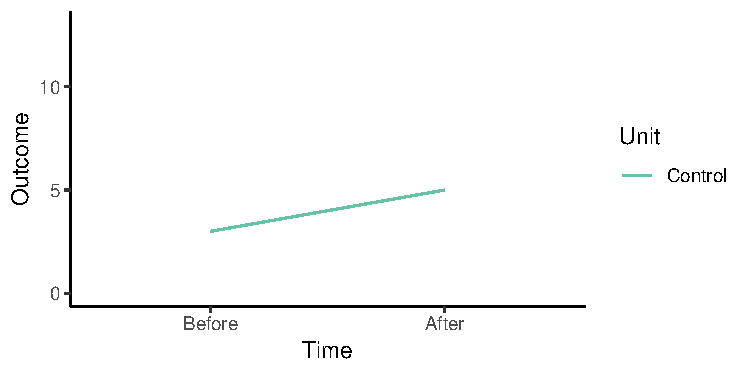
\includegraphics[width=\maxwidth]{figure/DinD_chart1-1} 

\end{knitrout}
\end{frame}


\begin{frame}
\frametitle{Difference-in-Differences}
\begin{knitrout}
\definecolor{shadecolor}{rgb}{0.969, 0.969, 0.969}\color{fgcolor}
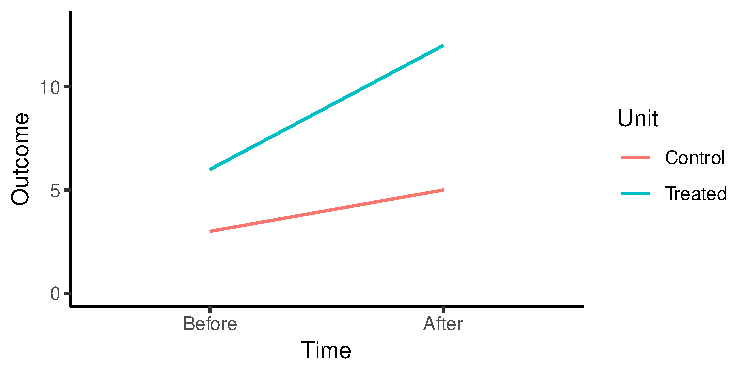
\includegraphics[width=\maxwidth]{figure/DinD_chart1b-1} 

\end{knitrout}
\end{frame}

\begin{frame}
\frametitle{Difference-in-Differences}
\begin{knitrout}
\definecolor{shadecolor}{rgb}{0.969, 0.969, 0.969}\color{fgcolor}
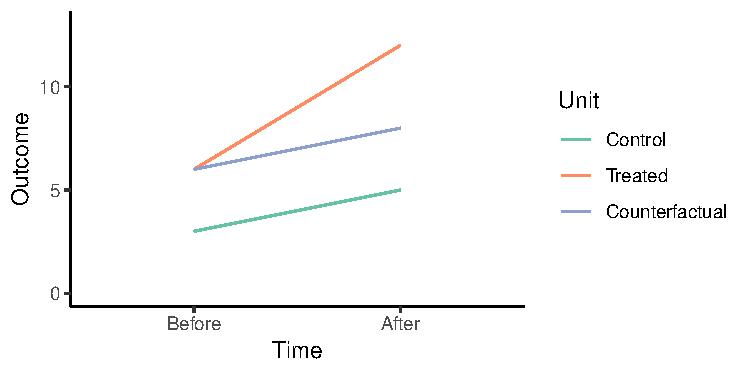
\includegraphics[width=\maxwidth]{figure/DinD_chart1c-1} 

\end{knitrout}
\end{frame}

\begin{frame}
\frametitle{Estimating Difference-in-Differences}
\begin{itemize}
\item Regression for the cross-unit effect of treatment
\end{itemize}
$$ Y_{it} = \alpha + \gamma D_i$$
\pause
\begin{itemize}
\item Regression for the before-after treatment comparison
\end{itemize}
$$ Y_{it} = \alpha + \gamma T_i$$
#pause
\begin{itemize}
\item The difference-in-differences estimate is just the \textit{interaction} of time and treatment status
\end{itemize}
$$ Y_{it} = \alpha + \gamma D_i + \delta T_t + \beta D_i * T_t $$
\begin{itemize}
\item $\beta$ is our \textbf{Average Treatment Effect} estimate
\end{itemize}
\end{frame}

\begin{frame}
\frametitle{Estimating Difference-in-Differences}
$$ Y_{it} = \alpha + \gamma D_i + \delta T_t + \beta D_i * T_t $$
\pause
\vspace*{10px}
$D=0, T=0: E(Y)=$ \pause $\alpha$ \\
\pause
$D=0, T=1: E(Y)=$ \pause $\alpha + \delta$ \\
\pause
$D=1, T=0: E(Y)=$ \pause $\alpha + \gamma$ \\
\pause
$D=1, T=1: E(Y)=$ \pause $\alpha + \delta + \gamma + \beta$ \\ \\
\vspace*{20px}
\pause
$\Delta(Y|D=1) = E(Y|D=1, T=1) - E(Y|D=1, T=0) =$ \pause $ \delta + \beta$ \\
\pause
$\Delta(Y|D=0) = E(Y|D=0, T=1) - E(Y|D=0, T=0) =$ \pause $ \delta$ \\
\pause
\vspace*{20px}
$\Delta(Y|D=1) - \Delta(Y|D=0) =$ \pause $\beta$
\end{frame}

\begin{frame}
\frametitle{Difference-in-Differences}
Raw Data:
\begin{knitrout}
\definecolor{shadecolor}{rgb}{0.969, 0.969, 0.969}\color{fgcolor}
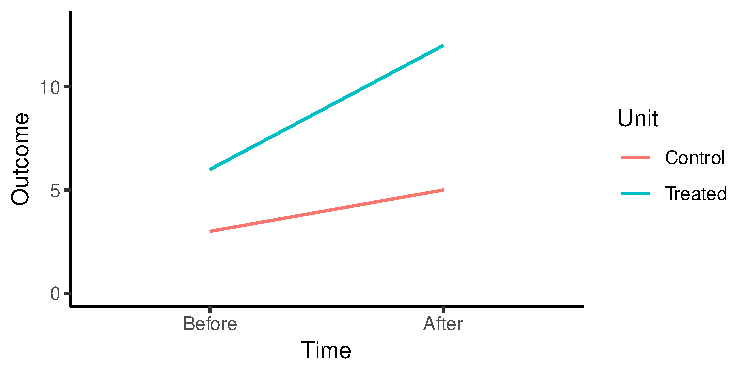
\includegraphics[width=\maxwidth]{figure/DinD_chart2-1} 

\end{knitrout}
\end{frame}

\begin{frame}
\frametitle{Difference-in-Differences}
Add a variable (fixed effect) for treated/control:
\begin{knitrout}
\definecolor{shadecolor}{rgb}{0.969, 0.969, 0.969}\color{fgcolor}
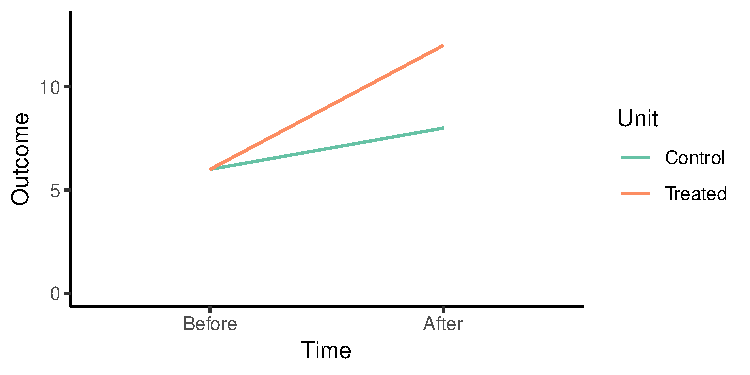
\includegraphics[width=\maxwidth]{figure/DinD_chart3-1} 

\end{knitrout}
\end{frame}

\begin{frame}
\frametitle{Difference-in-Differences}
Add a variable (fixed effect) for time:
\begin{knitrout}
\definecolor{shadecolor}{rgb}{0.969, 0.969, 0.969}\color{fgcolor}
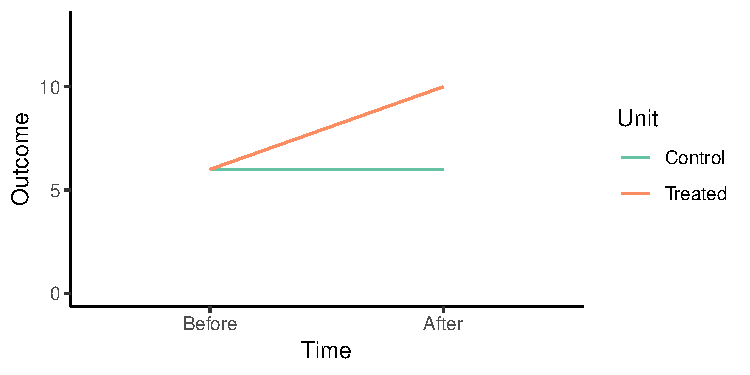
\includegraphics[width=\maxwidth]{figure/DinD_chart4-1} 

\end{knitrout}
\end{frame}

\begin{frame}
\frametitle{Difference-in-Differences}
Add a variable (fixed effect) for time:
\begin{knitrout}
\definecolor{shadecolor}{rgb}{0.969, 0.969, 0.969}\color{fgcolor}
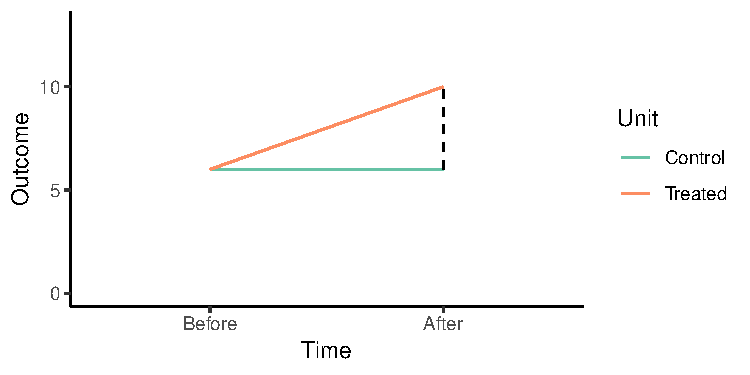
\includegraphics[width=\maxwidth]{figure/DinD_chart5-1} 

\end{knitrout}
\end{frame}

\begin{frame}
\frametitle{Estimating Difference-in-Differences}
\begin{itemize}
\item With time-series data, we haves temporal autocorrelation
\pause
\item So crucial to cluster standard errors by each cross-sectional unit (eg. each country)
\end{itemize}
\end{frame}

\begin{frame}
\frametitle{Difference-in-Differences}
\begin{itemize}
\item How do we know if there are \textbf{time-varying confounders}?
\pause
\item Selection into treatment is usually not just due to mostly 'fixed' variables (eg. gender) but due to 'time-varying' variables (eg. income, employment etc.)
\pause
\item Eg. training program participants' income has usually fallen a lot in the past few months
\pause
\item We want the outcome for the treated group to have the same trend as the control group
\pause
\item One test of this is to check if \textbf{pre-treatment trends are parallel}
\end{itemize}
\end{frame}

\begin{frame}
\frametitle{Difference-in-Differences}
\begin{knitrout}
\definecolor{shadecolor}{rgb}{0.969, 0.969, 0.969}\color{fgcolor}
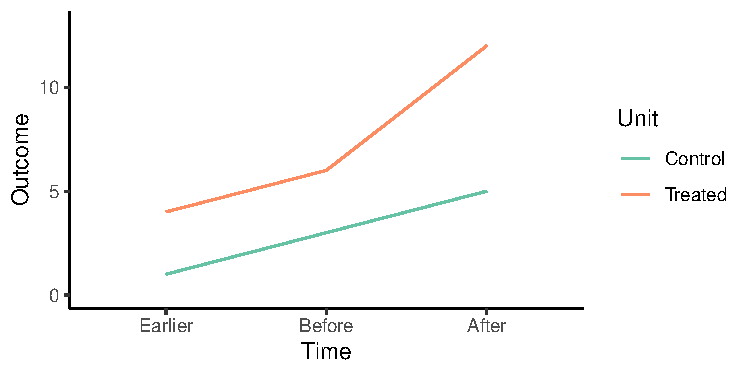
\includegraphics[width=\maxwidth]{figure/DinD_chart6-1} 

\end{knitrout}
\end{frame}

\begin{frame}
\frametitle{Difference-in-Differences}
\begin{knitrout}
\definecolor{shadecolor}{rgb}{0.969, 0.969, 0.969}\color{fgcolor}
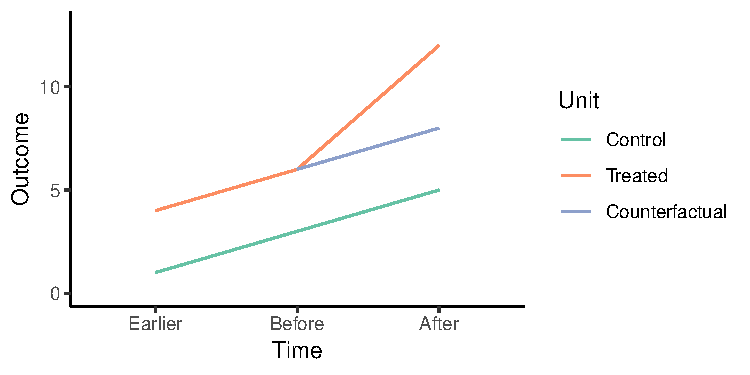
\includegraphics[width=\maxwidth]{figure/DinD_chart7-1} 

\end{knitrout}
\end{frame}

\begin{frame}
\frametitle{Assumptions}
\begin{enumerate}
\item Parallel pre-treatment trends between treated and control units
\pause
\item No compound treatment
\pause
\item No spillovers (SUTVA)
\pause
\item Group membership is stable (no migration from control to treatment)
\end{enumerate}
\end{frame}

\section{Chimeli and Soares 2017}

\begin{frame}
\frametitle{Chimeli and Soares 2017}
\begin{itemize}
\item How does an activity being illegal affect violence?
\pause
\item How did Brazil's ban on mahogany affect homicides?
\pause
\item What are the challenges to explanation?
\pause
\begin{itemize}
\item Omitted variables, eg. State capacity
\pause
\item Overall trends, eg. national decrease in homicides
\end{itemize}
\item Comparing the \textit{change} in violence in mahogany-growing areas to the change in violence in non-growing areas
\end{itemize}
\end{frame}

\begin{frame}
\frametitle{Chimeli and Soares 2017}
\begin{itemize}
\item In the 'After' period we need treated \textbf{and} control units 
\pause
\item But the ban on mahogany applied to \textbf{all} of Brazil.
\pause
\item So what are treatment and control here?
\pause
\item \textbf{Treatment:} \pause Municipalities with mahogany
\pause
\item \textbf{Control:} \pause Municipalities \textbf{without} mahogany
\pause
\item \textbf{Before:} \pause Pre-1998
\pause
\item \textbf{After:} \pause Post-1998
\pause 
\item \textbf{Outcome:} \pause Rate of Homicides
\end{itemize}
\end{frame}

\begin{frame}
\frametitle{Chimeli and Soares 2017}
\begin{itemize}
\item Multiple treatment timings:
\begin{itemize}
\item 1st policy change
\item 2nd policy change
\item Reverse treatment: Better policing of mahogany regulations
\end{itemize}
\end{itemize}
\end{frame}

\begin{frame}
\frametitle{Chimeli and Soares 2017}
\begin{itemize}
\item Methodology:
\pause
\end{itemize}
$$ Homicides_{it} = \gamma_t + \delta_i + \beta (Post-1998_t *  Mahogany_i) + \epsilon_i$$
\pause
\begin{itemize}
\item Cluster standard errors by municipality
\pause
\item Apply more complex state-specific trends for covariates to minimize risk of non-parallel trends
\pause
\item Supporting evidence: The 'extra' homicides were the type we'd expect from illegal activity
\end{itemize}
\end{frame}

\begin{frame}
\frametitle{Difference-in-Differences}
\begin{center}
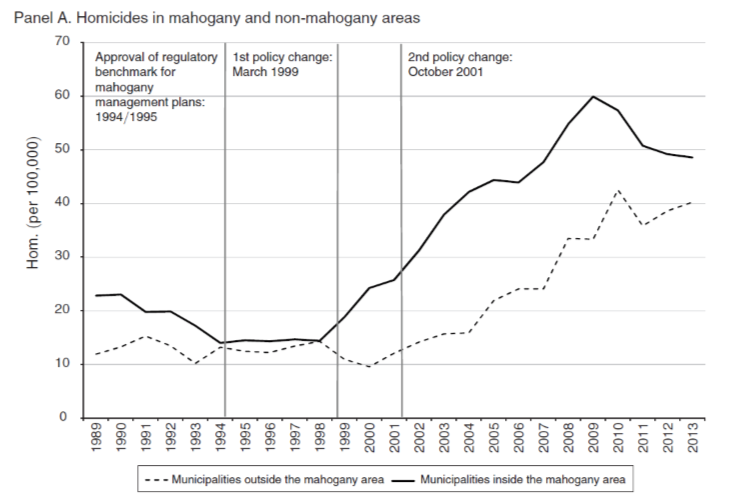
\includegraphics[scale=0.35]{Mahogany.png}
\end{center}
\end{frame}

\begin{frame}
\frametitle{Chimeli and Soares 2017}
\begin{itemize}
\item Interpretation
\begin{itemize}
\item Illegal activity prevents 'peaceful' contract enforcement
\item Competition between loggers
\item Contract enforcement with buyers
\item Intimidation of communities to not report logging
\end{itemize}
\end{itemize}
\end{frame}

\end{document}
